\documentclass[runningheads,a4paper]{llncs}

\usepackage{amssymb}
\setcounter{tocdepth}{3}
\usepackage{subfigure}
\usepackage{graphicx}
\usepackage{url}
\urldef{\mailsa}\path|{cherish, yhhan}@koreatech.ac.kr|
\newcommand{\keywords}[1]{\par\addvspace\baselineskip
\noindent\keywordname\enspace\ignorespaces#1}

\begin{document}

\mainmatter  % start of an individual contribution

% first the title is needed
\title{A Distributed Mobility Support in SDN-based LTE/EPC Architecture}

% a short form should be given in case it is too long for the running head
\titlerunning{DMM in SDN-based LTE/EPC Architecture}

% the name(s) of the author(s) follow(s) next
%
% NB: Chinese authors should write their first names(s) in front of
% their surnames. This ensures that the names appear correctly in
% the running heads and the author index.
%

\author{Yong-hwan Kim\inst{}
\and Hyun-kyo Lim\inst{}
\and Kyoung-han Kim\inst{}
\and Youn-Hee Han\inst{}}
%
\authorrunning{Yong-hwan Kim et al.}
% (feature abused for this document to repeat the title also on left hand pages)

% the affiliations are given next; don't give your e-mail address
% unless you accept that it will be published
\institute{Advanced Technology Research Center \\ Korea University of Technology and Education, Korea \\
\email{\{cherish, glenn89, goslim, yhhan\}@koreatech.ac.kr}}

%
% NB: a more complex sample for affiliations and the mapping to the
% corresponding authors can be found in the file "llncs.dem"
% (search for the string "\mainmatter" where a contribution starts).
% "llncs.dem" accompanies the document class "llncs.cls".
%

%\toctitle{Lecture Notes in Computer Science}
%\tocauthor{Authors' Instructions}
\maketitle


\begin{abstract}
As smart phone has rapidly proliferated over the past few years, LTE operators endeavor to cope with large mobile data traffic volumes.  To solve such problems, we propose a new SDN-based distributed mobility management supporting distributed P-GWs and centralized control plane in LTE/EPC networks. For enhancing network performance more, we also propose a route optimization strategy for internal traffic exchanged between LTE users. The proposed solutions' performance are compared with the conventional LTE/EPC network's scheme in terms of the P-GW data processing volume and the number of valid data sessions. The comparison results show that the proposed solution can be an efficient way to enhance the scalability of LTE/EPC core networks.

\keywords{Distributed Mobility Support, LTE/EPC, SDN}
\end{abstract}

\section{Introduction}
Due to the increasing popularity of smart-phones and other mobile devices, mobile data traffic is expected to highly increase. Accordingly, LTE operators are in urgent need of means to cope with such increase in data volumes. The evolution of mobile network architectures toward flat architectures is being considered as a key solution to cope with the explosion of mobile data traffic \cite{ref5}. For this, IETF Distributed Mobility Management (DMM) working group is trying to make standardizations of IP mobility anchors at an access network level \cite{ref6,ref7}. 

As 3GPP evolves to the Evolved Packet Core (EPC) network, the network hierarchy is also being flattened. In the hierarchy, the number of LTE/EPC network elements decreases, where the main elements in the data plane are Packet Data Network Gateway (P-GW), Serving Gateway (S-GW), and Evolved Node B (eNodeB). The number of hierarchy levels is reduced in the EPC network compared with the GPRS/UMTS network. In later deployment, P-GW and S-GW are expected to be co-located in the same physical element, thus the number of different network elements will be further reduced. In this hierarchy, P-GW provides access to Packet Data Network (PDN) by assigning an IP address to User Equipments (UEs) and serves as the mobility anchor point. UEs do not change their mobility anchor points if they remain attached to the same operator's access network. So, all data traffic for an UE is routed over P-GW and thus P-GW is needed to handle it.

As another trends in mobile networks, Software-Defined Networking (SDN) and Network Functions Virtualization (NFV) are being actively adopted by mobile operators. SDN and NFV can enable resource and service orchestration with dynamic provisioning by deploying and utilizing virtually-centralized control plane. In parallel with DMM technology, SDN and NFV will lead to the deployment of more flatter systems in which mobility anchor points can be placed closer to the UEs and the local breakout/traffic offload can be facilitated \cite{ref8}. Furthermore, a virtually centralized control plane leads to more flexibility by having the S-/P-GWs data-plane deployed in a distributed manner \cite{ref8-1}. It is however expected that the change of UE's mobility anchors upon handover will happen far more often due to high number of mobility anchors deployed at access networks. So, DMM should efficiently keep ongoing sessions active in case of handovers that require mobility anchor change. 

In this paper, we propose a new distributed LTE/EPC network architecture based on SDN and NFV supporting distributed P-GWs. It is designed based on the following requirements: 1) Distributing P-GWs closer to the UEs, 2) Virtually centralizing control plane, 3) Separation of the control and data planes, and 4) Efficient distributed mobility management. We also propose the route optimization for internal traffic exchanged by LTE/EPC UEs to enhance network performance. We have implemented the proposed solution on NS3-LENA simulation environment \cite{ref13-1}. The proposed solution's performance is compared with the conventional LTE/EPC network system's scheme in terms of the P-GW data processing volume and the number of valid data sessions. The comparison results show that the proposed LTE/EPC architecture and DMM solution can be a more efficient way to support the scalability of LTE/EPC core network.

The rest of this paper is organized as follows. Section 2 proposes a SDN-based DMM approach in LTE/EPC. Section 3 investigates the performance of our proposal by simulations, and Section 4 finally concludes this paper.

\begin{figure}[t]
\begin{center}
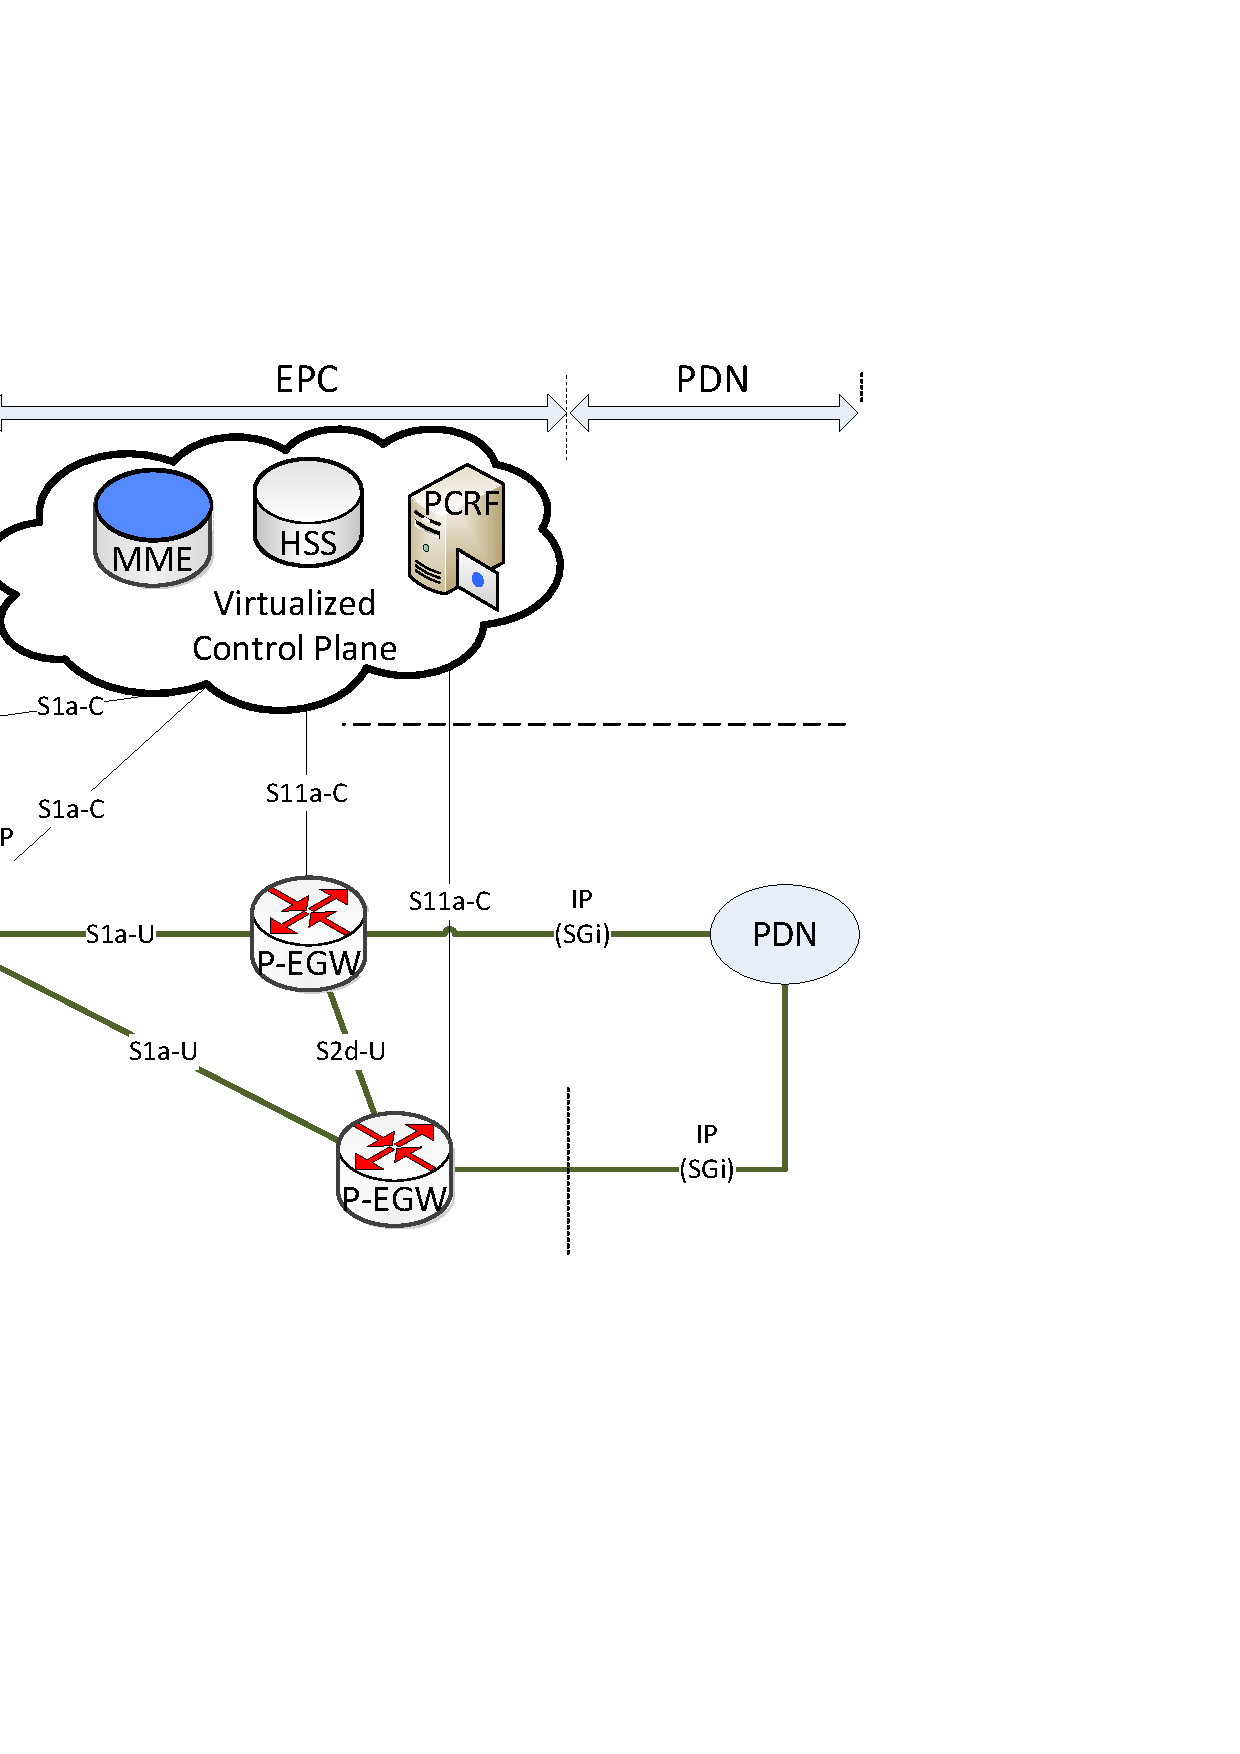
\includegraphics[width=8cm]{figures/fig1.pdf}
\end{center}\vspace{-0.6cm}
\caption{Reference model for SDN-based DMM architecture in LTE/EPC}
\label{fig:f1}\vspace{-0.6cm}
\end{figure}


\section{SDN-based Distributed Mobility Support}
\vspace{-0.2cm}
\subsection{SDN-based DMM architecture}
\vspace{-0.2cm}
Fig.\ref{fig:f1} shows the reference model for our SDN-based DMM (SDMM) architecture in LTE/EPC. As shown in the figure, multiple distributed components are deployed in different areas of the network, instead of employing a single centralized infrastructure based on P-GW,  A new network element named PDN edge gateway (P-EGW) is similar to the existing P-GW in term of the functionalities and the roles. However, P-EGWs will be deployed near to the radio area network (RAN), so that their location will be somewhere between eNB and S-GW. P-EGWs have also the role of SDN switches to communicate with the SDN controller deployed in virtually and centralized control plane. These distributed data plane allows scalability and flexibility to LTE/EPC networks.

The virtually control plane consists of much functions supported by Mobility Management Entity (MME), Home Subscriber Server (HSS), and Policy and Charging Rules Function (PCRF) which are control parts in conventional LTE/EPC networks. Such functions are deployed in a form of cloud system using NFV technology and can communicate with the entities in data plane via SDN technology. The centralized control plane can provide flexible and dynamic framework to LTE/EPC networks. In order to separate the LTE/EPC network's data and control planes, SDN technology is used to not only EPC core networks but also the edge network. The separation of the control and data planes allows sophisticated traffic management to be driven by software, rather than purely by hardware routers.

\begin{figure}[t]
\centering 
\subfigure[P-EGW1 $\longrightarrow$ P-GEW2]{
	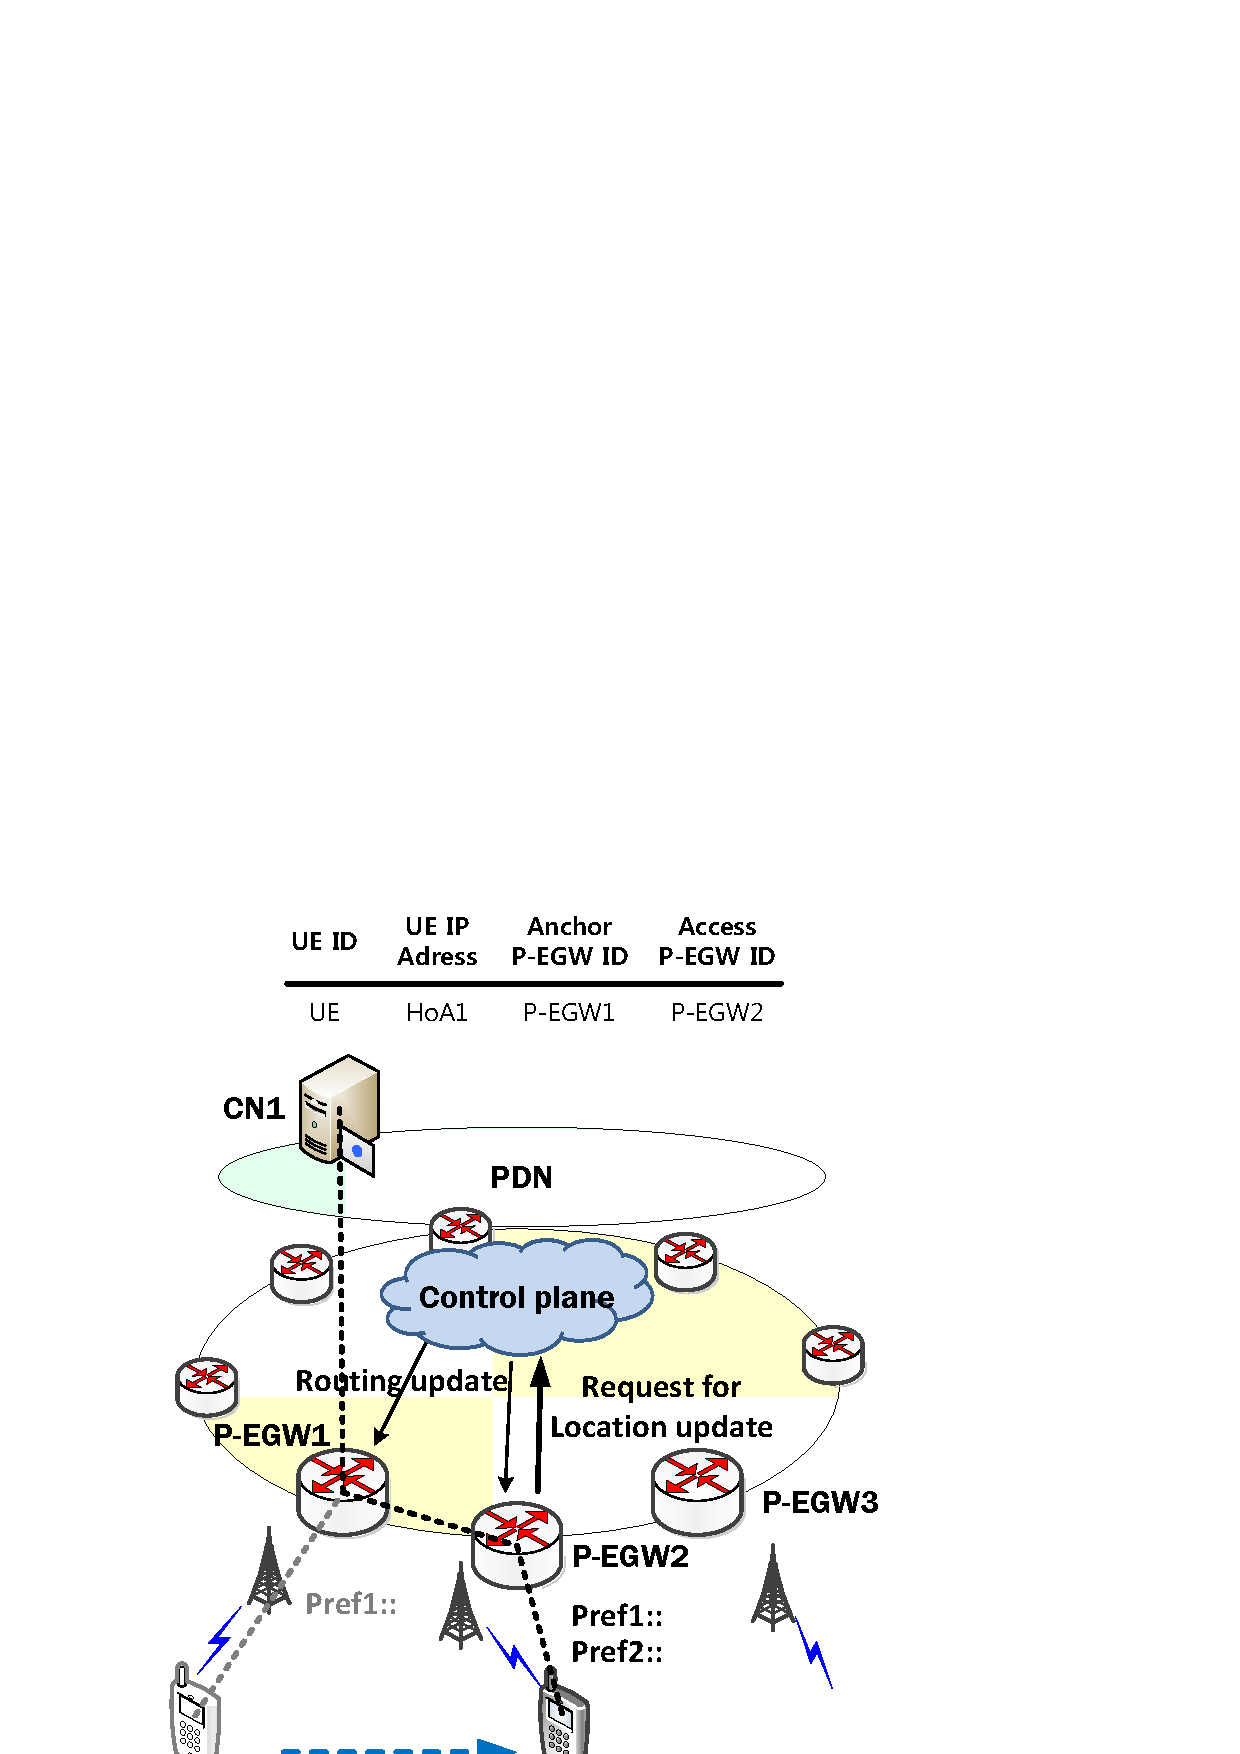
\includegraphics[width=0.40\linewidth, trim=0cm 0cm 0cm 0cm]{./figures/fig2(a).pdf}}
\subfigure[P-EGW2 $\longrightarrow$ P-GEW3]{
	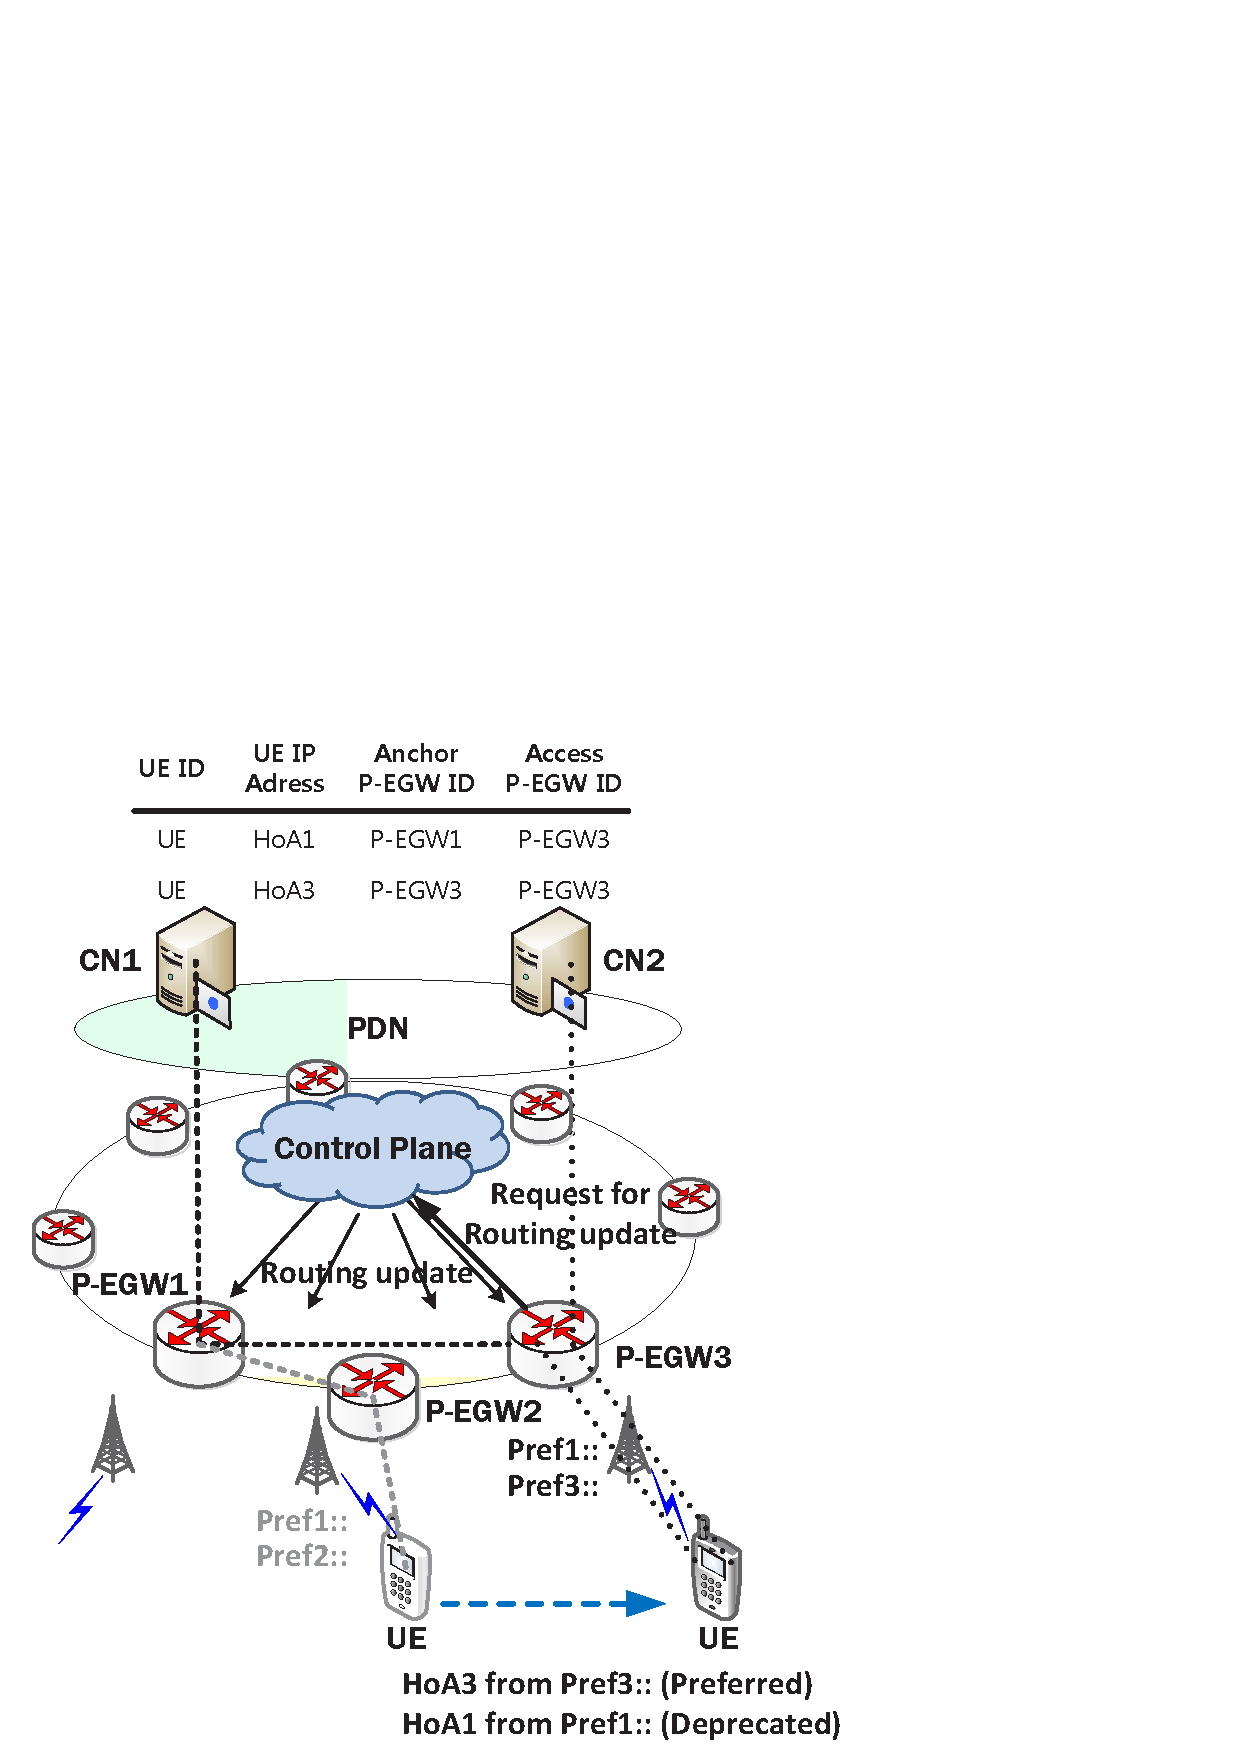
\includegraphics[width=0.44\linewidth, trim=0cm 0cm 0cm 0cm]{./figures/fig2(b).pdf}}\vspace{-0.3cm}
\caption{Procedure for UE movement in proposed SDMM}
\label{fig:2}\vspace{-0.6cm}
\end{figure}

\subsection{SDN-based DMM (SDMM)}
\vspace{-0.3cm}
In the proposed SDMM, there are two types of P-EGWs assigned to a PDN connection of an UE. The one is anchor P-EGW which plays a role of mobility anchor for the PDN connection, and the other is access P-EGW which maintains a normal Evolved Packet System (EPS) bearer for the PDN connection on the current location of the UE. 

When an UE initially attaches to an anchor P-EGW, it obtains an IP address called Home Address (HoA). When the UE moves and attaches to a different P-EGW (Access P-EGW), the access P-EGW finds out the address assigned to the UE during the authentication phase via SDN controller in the control plane. And then, a routing update between the anchor P-EGW and the access P-EGW is performed for session continuity by SDN controller in the control plane. In this way, the reachability of the UE is ensured while moving within the LTE/EPC network.

Meanwhile, when the UE in a new P-EGW's area tries to create a new PDN connection, the new P-EGW is in charge of creating the new PDN connection as anchor P-EGW. That is, an UE can have multiple PDN connections through different anchor P-EGWs. Therefore, these IP addresses related with multiple P-EGWs will be managed simultaneously in the UE. 

A location information of UE becomes $<$UE ID, UE IP Address, Anchor P-EGW ID, Access P-EGW ID$>$ per UE's PDN connection. UE IP Address is unique for PDN connection managed by anchor P-EGW. Anchor P-EGW ID and Access P-EGW ID are also needed to find the location of UE in distributed data plane. These location information of UE is managed by the control plane in a centralized manner and obtained by an entity in data plane through the mediation of SDN controller.

Examples of our solution are shown in Fig. \ref{fig:2}. In Fig. \ref{fig:2} (a), an UE initially attaches to P-EGW1 and starts to communicate with CN1 located in PDN. As explained previously, P-EGW1 becomes the anchor P-EGW for the PDN connection for this communication. When the UE moves to P-EGW2, which becomes an access P-EGW for the PDN connection, P-EGW2 acquires the UE's information via SDN controller in the control plane during the authentication phase. And then P-EGW2 requests for routing update to the control plane. When SDN controller in the control plane receives this request, it performs a routing update to SDN switches between anchor P-EGW1 and access P-EGW2. When the routing update is finished, the session data anchored P-EGW1 is redirected to P-EGW2. When the UE moves to P-EGW3 as shown in \ref{fig:2} (b), the session data anchored P-EGW1 is redirected to P-EGW3 though the same procedures. Meanwhile, when the UE creates a new session to CN2 located in PDN, P-EGW3 is the anchor P-EGW for the new session using a new IP address.

The data transferred after the movement of an UE in the proposed SDMM is routed through sub-optimal path, since the data should be redirected by an anchor P-EGW. However, the proposed SDMM can reduce the amount of signal messages related with routing update and the handover latency compared with the existing routing-based DMM approaches \cite{ref12}. Furthermore, it can remove the cost related with tunneling, while the tunneling cost is imposed on the existing host/network based DMM approaches \cite{ref7}.

An IP address assigned for a PDN connection managed by an LTE/EPC network operator can be made up based on a pre-defined prefix information. Therefore, if the IP address has such a pre-defined prefix, the data communication can be judged to be the one of inner traffic exchanged between UEs in the operator's network. In this case, the route for this data communication can be optimized by routing updates to SDN switches between the P-EGWs associated to such UEs.

%The proposed SDMM makes use of a routing protocol to support UE's mobility, instead of a tunneling protocol actively used in the existing IP mobility protocols. The routing protocol is running in the control plane centralized cloud form. The routing update message between the control plane and P-EGW having role of SDN switch will be exchanged via SDN technology. It can provide a selective routing update method.

\section{Performance Evaluation}

In this section, the proposed SDMM's performance is compared to the mobility management's one in the conventional LTE/EPC networks in terms of the P-GW data processing volume per unit time and the number of valid data sessions. For the analysis, we used the open source simulator NS-3.16 with the LENA LTE module (M4 release) \cite{ref13-1}.

The simulation area is $30 km \times 30 km$, where one P-GW, four S-GWs, and thirty-six eNBs are inter-connected in the conventional LTE/SAE network. On the other hand, twelve P-EGWs instead of P-GW and S-GWs are deployed for the proposed SDMM architecture. Each P-EGW is directly connected to three eNBs. Each wired link is a full-duplex link with $10 Gbps$ bandwidth. The delay of each link was configured to be a value between $25 ms$ and $125 ms$. The LTE wireless channel and modulation/encoding models are set to be the default models provided by NS-3.16-LENA. $100$ UEs are deployed randomly in the area and a voice over IP traffic is exchanged between UEs. A half of UEs sends 80 Bytes UDP data to the remaining UEs every 10ms, so that $64 Kbps$ codec is emulated in the simulation.

\begin{figure}[t] 
\centering 
\subfigure[Data throughput]{
	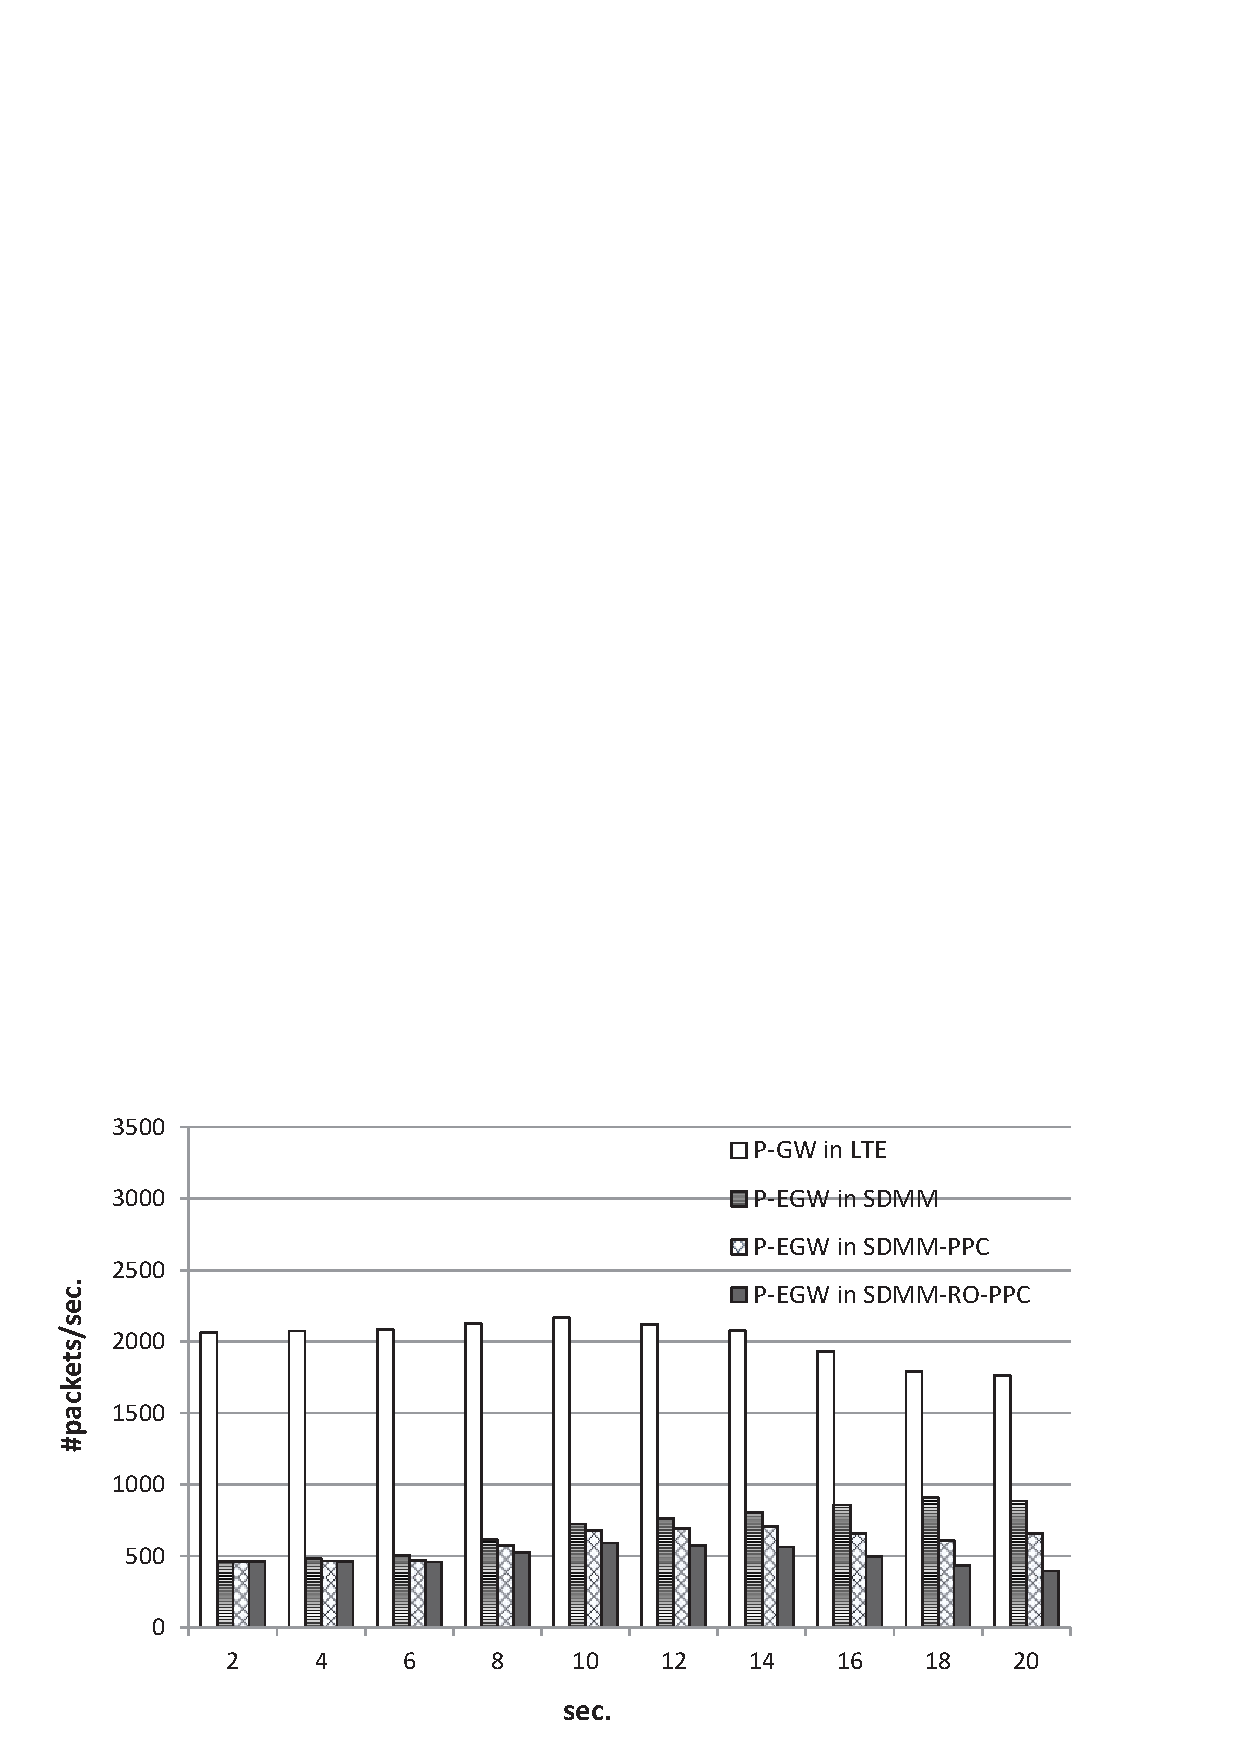
\includegraphics[width=0.47\linewidth, trim=0cm 0cm 0cm 0cm]{./figures/fig3.pdf}}
\subfigure[Number of valid data sessions]{
	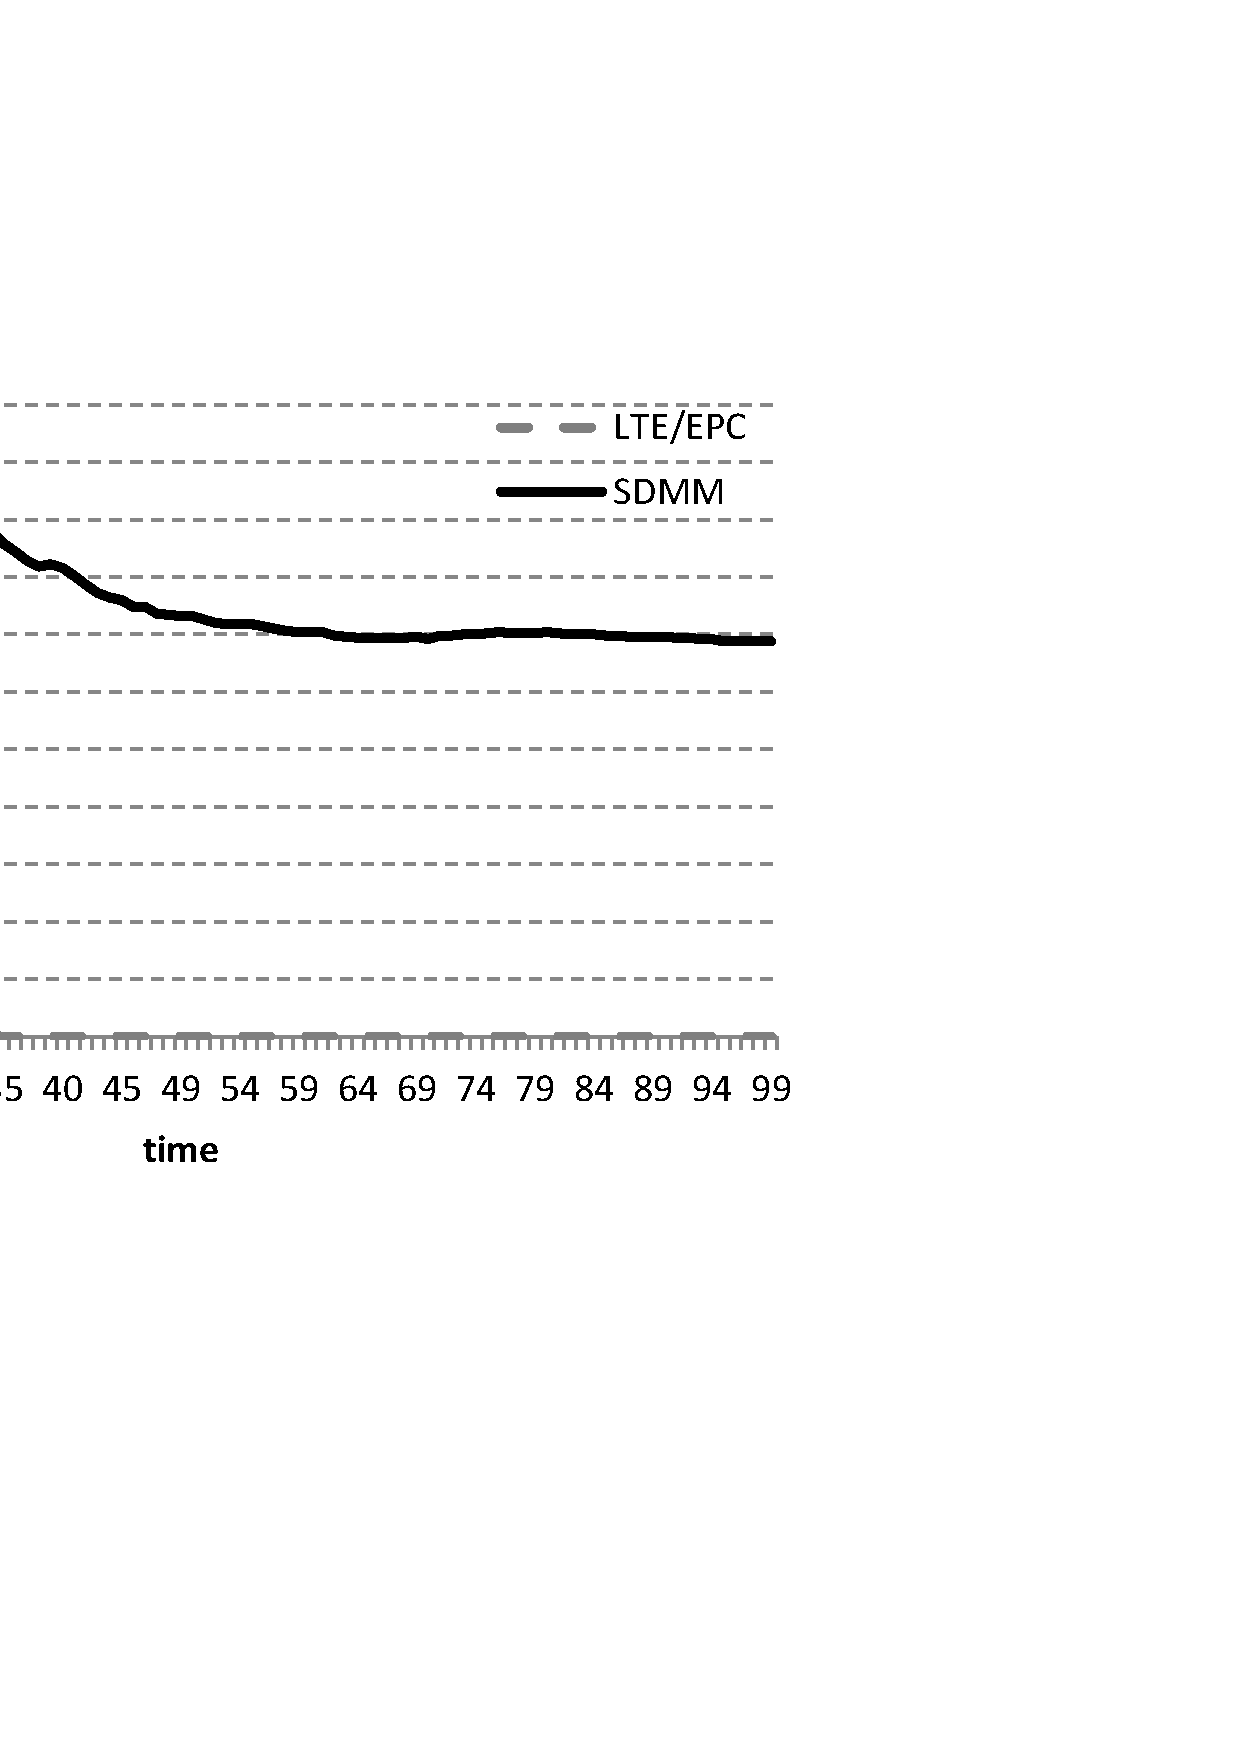
\includegraphics[width=0.49\linewidth, trim=0cm 0cm 0cm 0cm]{./figures/fig4.pdf}}\vspace{-0.3cm}
\caption{Performance evaluation}
\label{fig:3}\vspace{-0.6cm}
\end{figure}

Fig. \ref{fig:3} (a) shows the P-GW and the P-EGW's data processing volume per unit time over the given traffic scenario. The data processing volume observed at P-EGWs is apparently quite less than that at P-GW, due to the distributed architecture of P-EGWs. However, it is noted that the total amount of data processing volume observed at all P-EGWs is more than the one at P-GW. It is because more data traffic are redirected between P-EGWs. However, the data processing volume becomes low when the data traffic route is optimized.

Fig. \ref{fig:3} (b) plots the number of valid sessions observed in the conventional and proposed LTE/EPC networks. A session is valid in terms of service quality if its packet drop rate is lower than 10$\%$. In the experiment, we deployed stationary $100$ UEs randomly in the area and let each UE create a new session composed of 1Mbps UDP data traffic delivered to another UE every 40ms. As shown in the figure, the proposed SDMM scheme can create valid sessions twice more than the one used in the conventional LTE/EPC networks. Data traffic are concentrated to the P-GW in the conventional LTE/EPC network, while there is not such a single point in SDMM and all data traffic are directly routed between P-EGWs. That is, the SDMM scheme does not suffer from the bottleneck problem at a specific node in the network, and thus it is more scalable than the one of the conventional LTE/EPC networks. 

\section{Conclusions}


In this paper, a new SDN-based distributed LTE/EPC network architecture and DMM scheme called SDMM are proposed. P-EGWs' distribution close to LTE radio area networks can facilitate the traffic offload and perform local breakout as close as possible to UE, while reducing the load in LTE/EPC core network. Through our performance evaluation, we showed that the proposed ones become more efficient way to enhance the scalability of LTE/EPC core networks. In future, we will do more intensive simulation study in terms of signaling costs and handover latency.

\subsubsection*{Acknowledgments} This research was supported by the MSIP (Ministry of Science, ICT and Future Planning, 2014H1C1A1066391), Korea.

\begin{thebibliography}{4}

\bibitem{ref5} H. A. Chan, H. Yokota, J. Xie, P. Seite, D. Liu, "Distributed and Dynamic Mobility Management in Mobile Internet: Current Approaches and Issues," Journal of Communications, Vol 6, No 1, pp. 4-15, Feb. 2011

\bibitem{ref6} D. Liu, et al., "Distributed Mobility Management: Current Practices and Gap Analysis," IETF RFC 7429, Jan. 2015.

\bibitem{ref7} C. J. Bernardos, "PMIPv6-based Distributed Anchoring," IETF Internet Draft, draft-bernardos-dmm-distributed-anchoring-05, March 2015.

\bibitem{ref8} Y. Wang and J. Bi, "A Solution for IP Mobility Support in Software Defined Networks," In Proc. of 23rd ICCCN, 2014.

\bibitem{ref8-1} L. Valtulina, M. Karimzadeh, G. Karagiannis, G. Heijenk, and A. Pras, "Performance Evaluation of a SDN/OpenFlow-Based Distributed Mobility Management (DMM) Approach in Virtualized LTE Systems," In Proc of Globecom 2014 Workshop - Cloud Computing Systems, Networks, and Applications, 2014.

\bibitem{ref12} H. Chan and K. Pentikousis, "Enhanced Mobility Anchoring," IETF Internet draft, draft-chan-dmm-enhanced-mobility-anchoring-00 (work in progress), Jul. 2014.

\bibitem{ref13-1} LENA Design Documentation. http://lena.cttc.es/manual/lte-design.htm

\end{thebibliography}

\end{document}
